\chapter{Práctica 1: Puesta en Marcha y Calibración}

\begin{center}
  \small\renewcommand{\arraystretch}{1.3}
  \begin{tabular}{l l l l}
    \textbf{Equipo:}      & Robo R2   &
    \textbf{Actividades:} & 3 \\
    \textbf{Software:}    & Pantalla táctil RoboOS &
    \textbf{Duración:}    & 1,5 horas \\
  \end{tabular}
\end{center}

\section{Introducción}

Antes de la primera impresión hay que dejar la R2 lista: retirar el embalaje, conectarla a la red, actualizarla, calibrar la altura del hotend sobre la cama (\emph{Z-Offset}) y cargar filamento. Una calibración correcta es la causa principal de una buena primera capa; casi todos los problemas de adhesión nacen de un Z-Offset mal ajustado.

\begin{objetivebox}
\begin{itemize}
    \item Desembalar y preparar la impresora para su uso.
    \item Conectar y actualizar la impresora desde la pantalla táctil.
    \item Calibrar el Z-Offset con el asistente de la pantalla.
    \item Cargar filamento con el asistente de carga.
\end{itemize}
\end{objetivebox}

\vspace{6pt}

\begin{materialbox}
\begin{itemize}
    \item Impresora Robo R2 con su fuente, cable y tubo guía del filamento.
    \item Caja de herramientas (tapa del hotend, llaves allen, pinzas, tarjeta de calibración).
    \item Carrete de filamento PLA y tijeras.
    \item Red Wi-Fi o cable Ethernet.
\end{itemize}
\end{materialbox}

\vspace{6pt}

\begin{warningbox}
Con el hotend caliente no toque la boquilla ni el bloque calefactor. Durante la calibración mantenga las manos fuera de la zona de movimiento de la cama.
\end{warningbox}

\newpage
\section{Actividad 1: Desembalaje y configuración inicial}

\begin{enumerate}
    \item Abra las 3 pinzas inferiores de la caja y retire la cubierta superior. Corte la brida que sujeta la puerta y saque la caja de accesorios, retirando antes la cinta azul.
    \item Retire los \textbf{4 sujetadores naranjas} de las varillas (uno por esquina del carro superior) presionando el clip, y corte las bridas que sujetan las varillas a sus soportes.
    \item Quite la cinta azul que sujeta las partes móviles y levante la impresora por las asas inferiores.
    \item Coloque la \textbf{tapa del hotend} (se sujeta con imanes) y conecte el cable de alimentación a la parte trasera y a la red eléctrica.
    \item Encienda la impresora.
    \item Conecte a Wi-Fi: \ruta{Utilities}\flecha\ruta{Network}\flecha\ruta{Configure Wifi}, elija su red, escriba la clave con el teclado en pantalla y pulse \ruta{Connect}. También puede usar un cable Ethernet.
    \item Actualice: \ruta{Utilities}\flecha\ruta{Update}. Si ya está al día, el botón aparece en gris con la leyenda \emph{up to date}. La actualización tarda cerca de un minuto.
\end{enumerate}

\begin{infobox}[Guarde el embalaje]
Conserve la caja y las espumas: pueden hacer falta para el transporte o para hacer válida la garantía. El fabricante recomienda también registrar el equipo para servicio y garantía.
\end{infobox}

\begin{figure}[H]
    \centering
    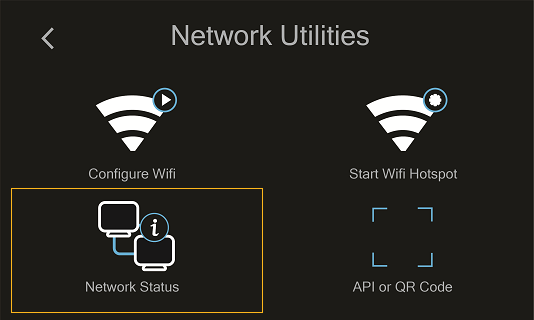
\includegraphics[width=0.5\linewidth]{r2_network.png}
    \caption{Menú \emph{Network Utilities}: configurar Wi-Fi, modo hotspot, estado de red y código QR.}
    \label{fig:network}
\end{figure}

\newpage
\section{Actividad 2: Calibración del Z-Offset}

El \textbf{Z-Offset} es la distancia entre la boquilla y la cama cuando la cama está en su posición de origen (abajo). Puede cambiar si la cama no queda bien asentada o si el hotend se desplaza.

\subsection*{Asistente Z-Offset}

\begin{enumerate}
    \item \ruta{Utilities}\flecha\ruta{Wizards}\flecha\ruta{Z-Offset Wizard}. La impresora se lleva a su posición de origen.
    \item Con las flechas \textbf{arriba/abajo} mueva la cama mientras desliza la \textbf{tarjeta de calibración} (o una hoja de papel) entre la boquilla y la cama.
    \item Deténgase cuando sienta una \textbf{ligera resistencia}: la tarjeta debe poder moverse, pero tocando a la vez la boquilla y la cama. Si la cama está tan alta que la tarjeta no pasa, baje con la flecha hasta que pase con un leve roce.
    \item Pulse \ruta{Finished}; la impresora calcula y guarda el valor. Pulse \ruta{Finished} otra vez para cerrar.
\end{enumerate}

\subsection*{Ajuste fino (Fine Tune Offset)}

Si la boquilla arrastra sobre la cama (Z muy bajo) o la pieza no se pega (Z muy alto), use \ruta{Utilities}\flecha\ruta{Wizards}\flecha\ruta{Fine Tune Offset}. La impresora imprime líneas de prueba y usted sube o baja el valor entre pasadas.

\begin{warningbox}[Antes del ajuste fino]
Nivele la cama con los tornillos de mariposa inferiores antes de iniciar este asistente; de lo contrario, el resultado no es confiable.
\end{warningbox}

\begin{enumerate}
    \item Elija el material cargado y la esquina desde la que empezará a imprimir las líneas.
    \item En la pantalla \emph{Adjust Offset} elija el incremento, use \ruta{Test Offset} y compare con la imagen de referencia.
    \item Cuando el resultado sea satisfactorio, pulse la flecha de avance (arriba a la derecha) y \ruta{Save}.
\end{enumerate}

\begin{infobox}[Ajuste manual (avanzado)]
Se puede editar el valor en \ruta{Utilities}\flecha\ruta{Options}\flecha\ruta{EEPROM}\flecha\ruta{Home Offset}. Un valor \textbf{menor} acerca la cama a la boquilla; uno \textbf{mayor} la aleja. Si el valor es cercano pero la pieza no se pega, pruebe cambios de 0,1 a 0,2~mm.
\end{infobox}

\newpage
\section{Actividad 3: Carga de filamento}

\begin{enumerate}
    \item Desenganche el soporte del carrete empujando la palanca superior desde la parte trasera, e inserte el tubo guía en el bloque del sensor de filamento.
    \item Cuelgue el carrete en el soporte superior, desenrolle al menos \textbf{30~cm} de filamento y \textbf{corte la punta} con tijeras.
    \item Pase el filamento por la base del bloque del sensor y por el tubo guía hasta el extrusor. El filamento \textbf{debe pasar por el bloque del sensor} (si no, el sensor marcará error de falta de filamento).
    \item Presione la palanca del extrusor y guíe el filamento hasta los engranajes.
    \item \ruta{Utilities}\flecha\ruta{Wizards}\flecha\ruta{Filament Loading Wizard}. La impresora calienta; cuando termine, el engranaje empuja el filamento hasta la boquilla.
    \item Cuando vea salir plástico por la boquilla pulse \ruta{Next} y luego \ruta{Done}.
\end{enumerate}

Para \textbf{descargar} el filamento use \ruta{Utilities}\flecha\ruta{Wizards}\flecha\ruta{Filament Change Wizard}: tras calentar, el engranaje retrae el filamento hasta que sale por la parte superior del extrusor.

\begin{infobox}[Cambio de material]
Si cambia de ABS a PLA, caliente el hotend a temperatura de ABS y empuje un poco de PLA para sacar todo el ABS. Después baje a la temperatura del PLA; de lo contrario, la boquilla puede taparse.
\end{infobox}

\section{Entregables}

\begin{entregabox}
\begin{itemize}
    \item Fotografía de la impresora lista (sin sujetadores de embalaje, con tapa del hotend) y captura de la pantalla \emph{up to date}.
    \item Valor de Z-Offset obtenido y breve descripción de cómo se comprobó (tarjeta o papel).
    \item Fotografía del filamento saliendo por la boquilla.
\end{itemize}
\end{entregabox}
